\documentclass[journal]{IEEEtran}

%\usepackage[brazilian]{babel}

\makeatletter
%\adddialect\l@BRAZILIAN\l@brazilian
\makeatother


\usepackage[T1]{fontenc}
\usepackage[utf8]{inputenc}
\usepackage{lmodern}

\usepackage{ae}
\usepackage{hyphenat}
\usepackage{fancyhdr}
\usepackage{float}
\usepackage{cite}
\usepackage[pdftex]{hyperref}
\usepackage[pdftex]{color,graphicx}

\usepackage[cmex10]{amsmath}

\usepackage{array}

\usepackage{mdwmath}
\usepackage{mdwtab}
\usepackage{url}
\usepackage{tikz}

\hyphenation{op-tical net-works semi-conduc-tor con-si-de-ram fa-mi-lia-ri-za-ção}
\hypersetup{colorlinks, citecolor=black, filecolor=black, linkcolor=black, urlcolor=blue}

%Algoritmos
\usepackage[english]{algorithm2e}

\begin{document}
\title{Introduction to Numeric Simulation of Magnetic Fluid Flows}

\author{Ataias~Pereira~Reis, Yuri~Dumaresq~Sobral, Francisco~Ricardo~da~Cunha\\Universidade de Brasília\\Departamento de Matemática\\Brasília, Brasil\\ataiasreis@gmail.com}

% The paper headers
\markboth{Scientific Initiation Program, July~2015}%
{Shell \MakeLowercase{\textit{et al.}}: Bare Demo of IEEEtran.cls for Journals}

\maketitle


\begin{abstract}
%\boldmath
This work aims at studying how magnetic fluids behave in a 2D lid-driven cavity. In order to achieve this goal, a computer program was developed to solve the Navier Stokes equation using finite differences. In addition to that, models of the magnetostatic force were introduced. Solving the Poisson equation is done by means of an implicit method with sparse matrices and Cholesky factorization. Once the hydrodynamic and magnetostatic parts are solved, vector fields and streamlines are plotted for analysis of the flow. A few distinct Reynolds numbers are tested, as well as some different magnetic parameters. The governing equations in continuous form and also in discrete form are presented, as well as the vectors fields resulted from computations.
\end{abstract}
% IEEEtran.cls defaults to using nonbold math in the Abstract.
% This preserves the distinction between vectors and scalars. However,
% if the journal you are submitting to favors bold math in the abstract,
% then you can use LaTeX's standard command \boldmath at the very start
% of the abstract to achieve this. Many IEEE journals frown on math
% in the abstract anyway.

% Note that keywords are not normally used for peerreview papers.
\begin{IEEEkeywords}
Magnetic fluids, Navier~Stokes, PDE, Poisson, Laplace, Finite~differences
\end{IEEEkeywords}

% For peer review papers, you can put extra information on the cover
% page as needed:
% \ifCLASSOPTIONpeerreview
% \begin{center} \bfseries EDICS Category: 3-BBND \end{center}
% \fi
%
% For peerreview papers, this IEEEtran command inserts a page break and
% creates the second title. It will be ignored for other modes.
\IEEEpeerreviewmaketitle

\section{Introduction}
This project aims at studying magnetic fluids in a 2D lid-driven cavity. The ideal cavity used here is a square of side equal to unity. All the boundaries but the top are with null velocities. The lid has a stationary velocity pattern that will be presented. Even though this may seem a simplistic method, papers have been presented not only in the last century but also in this century to study real problems. Garandet \cite{Garandet2012149} uses a similar approach to study solute segregations. On the field of biomagnetic fluids, Tzirtzilakis \cite{Tzirtzilakis2013} has also considered a cavity and analysed the stationary solutions under different conditions of the Reynolds numbers and magnetic parameters. Differently from this last researcher, our project has not considered a method to find directly the steady state, but has evolved in discrete time steps from time 0 to an end time defined. The advantage is that animations can be created to show how the flow evolves. 

\section{Governing Equations}
Equations \ref{navierstokes} and \ref{navierincompressibilidade} govern the flow of an incompressible fluid. The first one is the Navier Stokes equation, while the second one is the condition for incompressibility.

\begin{eqnarray}
\rho\left( \frac{\partial {\textbf{v}}}{\partial t}+\textbf{v}\cdot\nabla \textbf{v} \right)=-\nabla p+\mu\nabla^2 \textbf{v} + \textbf{f}\label{navierstokes}\\
\nabla\cdot\textbf{v}=0\label{navierincompressibilidade}
\end{eqnarray}

Computer solutions require certain conditions on the time step and spacing of grid points. The requirements are: stable diffusion, Equation \ref{stablediffusion}; stable advection, Equation \ref{stableadvection} and hydrodynamic boundary layer, Equation \ref{boundarylayer}. $U$ is the maximum speed in the cavity. If those equations are not satisfied, the solution will be wrong as the program may be trying to solve faster than the laws of physics allow. The program may not even converge and stay on an infinite loop.

\begin{eqnarray}
\Delta t &<& \frac{1}{4}\mathit{Re}\Delta x^2 \label{stablediffusion}\\
\Delta t &<& \frac{\Delta x}{U} \label{stableadvection}\\
\Delta x &<& \frac{1}{\mathit{Re}} \label{boundarylayer}
\end{eqnarray}

The Navier Stokes equation is thorough, encompassing several types of flow. A specific solution is found by specifying its boundary conditions. For the current work, the conditions are

\begin{eqnarray}
u(x,1) & = & \sin^2(\pi x),\\
u(x,0) & = & u(0,y) = u(1,y) = 0\\
v(x,0) & = & v(x,1) = v(0, y) = v(1, y) = 0
\end{eqnarray}

Besides the hydrodynamics equations and conditions, the magnetic force - $\mathbf{f}$ - must be computed. From Maxwell's theory, Equations \ref{firstmagneticequation} and \ref{secondmagneticequation} are obtained. 

\begin{eqnarray}
\mathbf{B} &=& \mu_0(\mathbf{M}+\mathbf{H})\label{firstmagneticequation}\\
\nabla\cdot \mathbf{B} & = & 0\label{secondmagneticequation}
\end{eqnarray}

From the latter equations, it is possible to conclude that 

\begin{eqnarray}
\nabla\cdot \mathbf{M} = -\nabla\cdot\mathbf{H}	\label{mh1}.
\end{eqnarray}

The magnetostatic regime implies $\nabla\times \mathbf{H} = \mathbf{0}$ which indicates there is a potential field $\phi$ that satisfies $\mathbf{H} = -\nabla \phi$. With these last equations, it is possible to obtain Equation \ref{eqcampomag}. This is a Poisson equation that will give $\phi$ according the the applied field $\mathbf{H}$. The superparamagnetic case is being considered, what implies $\mathbf{M} = \chi \mathbf{H}$.

\begin{eqnarray}
\nabla^2\phi &=& \nabla\cdot \mathbf{M}\label{eqcampomag}
\end{eqnarray}

Nevertheless, the potential $\phi$ cannot be introduced directly in the Navier Stokes equation. What is needed is a relation that gives the magnetic force, which could then be incorporated in the fluid equations. Equation \ref{magneticforce} stands for the magnetic force, while Equation \ref{cpm} is the magnetic reynolds number.

\begin{eqnarray}
\mathbf{f} & = & \mathrm{Cpm} \mathbf{M}\cdot \nabla \mathbf{H}\label{magneticforce}\\
\mathrm{Cpm} & = & \frac{\mu_0 H_0^2}{\rho u^2}\label{cpm}
\end{eqnarray}


One thing that is missing is the boundary conditions for the potential field $\phi$. To understand how they are derived, first consider an applied magnetic field $\mathbf{H}$. A condition that is imposed is continuity of the normal component of $\mathbf{B}$ - $\mathbf{B}$ can be obtained by Equation \ref{firstmagneticequation}. This continuity can be mathematically represented by Equation \ref{normalconditionB}. From this, Equation \ref{normalConditionB2} can be obtained.

\begin{eqnarray}
\left(\mathbf{B}_{\mathrm{out}} - \mathbf{B}_{\mathrm{in}}\right)\cdot \mathbf{n} &=& 0 \label{normalconditionB}\\
\mu_0 (H_{\mathrm{out}}^{\mathrm{n}} + M_{\mathrm{out}}^{\mathrm{n}}) &=&  \mu_0(H_{\mathrm{in}}^{\mathrm{n}}+M_{\mathrm{in}}^{\mathrm{n}})\label{normalConditionB2}
\end{eqnarray}

\section{Solution Method}

In order to solve the flow with a computer, the latter equations should be expanded to its 2D form and then discretized. Nevertheless, the fluid flow equation is highly non-linear due to its convective term - $\mathbf{v}\cdot \nabla \mathbf{v}$. Another problem is that the pressure needed at each time step is not known and need to be solved. The pressure is needed to know the velocity and the velocity is needed to obtain the pressure. To solve this dilemma, the Chorin method \cite{Chorin1997118} was used. This method is the time splitting. To understand this method, one can start by using finite differences for the velocity derivative with respect to time and then doing a smart manipulation with two new terms. This is presented in Equation \ref{vdottimesplitting}.

\begin{equation}
\frac{\partial \textbf{v}}{\partial t}\approx \frac{\textbf{v}^{n+1}-\textbf{v}^n}{\Delta t}=\frac{\textbf{v}^{n+1}-\textbf{v}^*}{\Delta t}+\frac{\textbf{v}^{*}-\textbf{v}^n}{\Delta t} \label{vdottimesplitting}
\end{equation}

The idea of time-splitting is to impose each parcel of Equation \ref{vdottimesplitting} to a different part of the Navier Stokes equation. The last term in the right hand side is used to solve Equation \label{equacaovestrela}, in which pressure is not considered, while the term just before it is used to obtain the next time step from the pressure calculated with $\mathbf{v}^{*}$.

\begin{eqnarray}
\frac{\textbf{v}^{*}-\textbf{v}^n}{\Delta t}&=& \nu\nabla ^2 \textbf{v} + \frac{\textbf{f}}{\rho} - \textbf{v}\cdot \nabla \textbf{v}\label{equacaovestrela}\\
\frac{\textbf{v}^{n+1}-\textbf{v}^*}{\Delta t}&=&-\frac{1}{\rho}\nabla p\label{equacaoprepressao}
\end{eqnarray}




\begin{figure}[!ht]
\centering
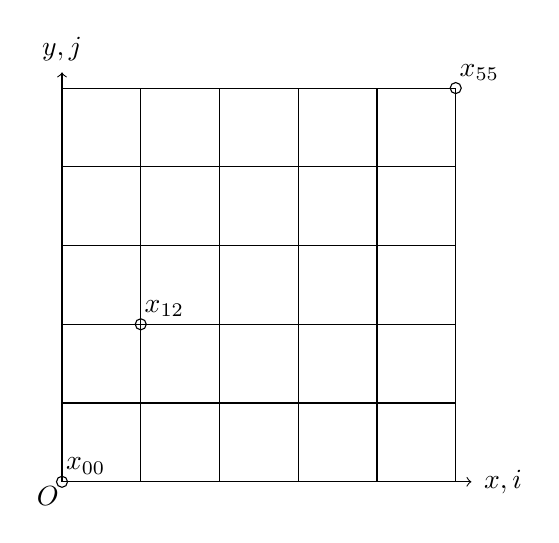
\begin{tikzpicture}
%grid
\draw (0,0) grid +(5,5);

%axes
\draw[->] (0,0) -- (xyz cs:x=0, y=5.2);
\draw (0,5.5) node {$y,j$};

\draw[->] (0,0) -- (xyz cs:x=5.2,y=0);
\draw (5.6,0) node {$x,i$};
\draw (-0.18,-0.18) node {$O$};

\draw (0.3,0.2) node {$x_{00}$};
\draw (0,0) circle (2pt);

\draw (5.3,5.2) node {$x_{55}$};
\draw (5,5) circle (2pt);

\draw (1.3,2.2) node {$x_{12}$};
\draw (1,2) circle (2pt);
\end{tikzpicture}
\caption{Malha padrão para discretizar Laplace e Poisson\label{malha_poisson}}
\end{figure}


Pelo fato deste primeiro método abordado ser iterativo, com um \textit{loop} sendo executado até a convergência ser obtida, é natural escolher um método de parada. Isto poderia ser: (1) escolher um tempo limite de execução, (2) ver a diferença entre duas matrizes após uma iteração completa em seus pontos internos, para analisar se a diferença entre elas é desprezível e se indica convergência, ou ainda (3) pode-se calcular a Equação \ref{laplace_discreta_zero} em cada ponto interno, que seria o melhor a se fazer, e analisar se a equação está dentro de uma faixa de erro desejada. No Algoritmo \ref{algo_laplace_iter}, é apresentada a formulação inicial utilizada.

\begin{algorithm}
\SetKwInOut{Input}{input}\SetKwInOut{Output}{output}
\Input{Matriz $n\times n$ com as condições de contorno de Dirichlet}
\Output{Matriz com a solução da equação de Laplace}
\BlankLine
$STOP=0$\;
$err \leftarrow 10^{-6}$\;
\While{$STOP \neq 1$}{\label{InRes1}
$u^{\textrm{old}}\leftarrow u$\;

\For{$i\leftarrow 1$ \KwTo $n-2$}{
\For{$j\leftarrow 1$ \KwTo $n-2$}{\label{forins}
$u_{ij}\leftarrow (u_{i+1j}+u_{i-1j}+u_{ij+1}+u_{ij-1})/4$\;
}
}
$ERROR\leftarrow Norma(u^{\textrm{old}}-u)$\;

\If{$ERROR < err$}{
$STOP\leftarrow1$\;
}
}

\caption{Resolvendo a equação de Laplace Iterativamente}\label{algo_laplace_iter}
\end{algorithm}

O conjunto das Equações \ref{first_implicit} a \ref{last_implicit} é um sistema linear, e é possível representá-lo na forma matricial $Ax = b$. O que torna este problema interessante é que a matriz $A$ e o vetor $b$ tem padrões muito bem definidos. A matriz $A$ segue o padrão apresentado na Equação \ref{matriz_a}.

\begin{equation}
\left( \begin{array}{ccccccccc}
-4 & 1 & 0 & 1 & 0 & 0 & 0 & 0 & 0 \\ % 1
1 & -4 & 1 & 0 & 1 & 0 & 0 & 0 & 0 \\ % 2
0 & 1 & -4 & 0 & 0 & 1 & 0 & 0 & 0 \\ % 3
1 & 0 & 0 & -4 & 1 & 0 & 1 & 0 & 0 \\ % 4
0 & 1 & 0 & 1 & -4 & 1 & 0 & 1 & 0 \\ % 5
0 & 0 & 1 & 0 & 1 & -4 & 0 & 0 & 1 \\ % 6 
0 & 0 & 0 & 1 & 0 & 0 & -4 & 1 & 0 \\ % 7
0 & 0 & 0 & 0 & 1 & 0 & 1 & -4 & 1 \\ % 8
0 & 0 & 0 & 0 & 0 & 1 & 0 & 1 & -4 \\ % 9
\end{array} \right) \label{matriz_a}
\end{equation}

Observando o padrão de formação da matriz $A$ pentadiagonal e também o padrão do vetor $b$, obtém-se um sistema linear cuja incógnita são os pontos internos $x$. A solução é $x=A^{-1}b$.

Como se nota, a resolução é direta, mas o algoritmo para se resolver este sistema linear pode ser muito mais complexo. Mas há um problema para este método, que um sistema pode ficar extremamente grande com um $n$ relativamente pequeno, tão grande, ao ponto de necessitar de mais memória do que o computador tem. Isso se resolve utilizando matrizes esparsas, que só salvam na memória elementos diferentes de zero. A matriz $A$ é uma matriz esparsa, na qual a maioria de seus elementos é igual a 0. Utilizaram-se métodos prontos para resolução de sistemas esparsos da biblioteca Eigen. A Figura \ref{pontos_vs_tempo_direto} mostra a relação entre tempo e número de pontos para o método direto. Note que o tempo é muito menor que nos métodos iterativos, nas Figuras \ref{pontos_vs_tempo_1th} e \ref{pontos_vs_tempo_4th}.

\section{Results}

\begin{figure}[!ht]
\centering
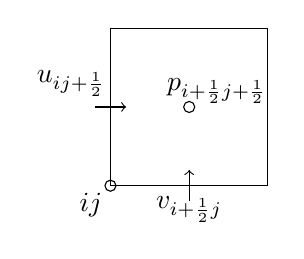
\begin{tikzpicture}
\draw (0,0) rectangle (2,2);
\draw (1.35,1.2) node {$p_{i+\frac{1}{2}j+\frac{1}{2}}$};
\draw[->] (1,-0.2) -- (1,0.2);
\draw (1,-0.3) node {$v_{i+\frac{1}{2}j}$};
\draw[->] (-0.2,1) -- (0.2,1);
\draw (-0.5,1.3) node {$u_{ij+\frac{1}{2}}$};
\draw (1,1) circle (2pt);

\draw (0,0) circle (2pt);
\draw (-0.25,-0.25) node {$ij$};
\end{tikzpicture}
\caption{Elemento de malha escalonada}
\end{figure}

\begin{figure}[!ht]
\centering
\tikzstyle{help lines}+=[dashed]% aaarghhh!!!
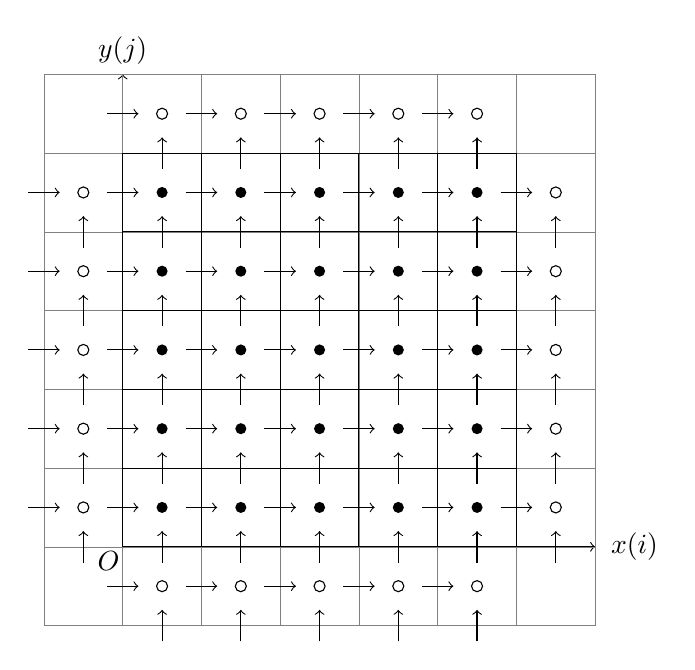
\begin{tikzpicture}
%axes
\draw[->] (0,5) -- (xyz cs:y=6);
\draw (0,6.3) node {$y(j)$};
\draw[->] (5,0) -- (xyz cs:x=6);
\draw (6.5,0) node {$x(i)$};
\draw (-0.18,-0.18) node {$O$};
%grid
\draw[style=help lines] (-1,-1) grid +(7,7);
\draw (0,0) grid +(5,5);
%internal p points
\foreach \x in {0.5,1.5,2.5,3.5,4.5}
  \foreach \y in {0.5,1.5,2.5,3.5,4.5}
  {
  \fill (canvas cs:x=\x cm,y=\y cm) circle (2pt);
}
%External p points
\foreach \x in {0.5,1.5,2.5,3.5,4.5}
  \draw (\x,-0.5) circle (2pt);
\foreach \y in {0.5,1.5,2.5,3.5,4.5}
  \draw (5.5,\y) circle (2pt);
\foreach \y in {0.5,1.5,2.5,3.5,4.5}
  \draw (-0.5,\y) circle (2pt);
\foreach \x in {0.5,1.5,2.5,3.5,4.5}
  \draw (\x,5.5) circle (2pt);
%Internal Horizontal Velocities Points
\foreach \x in {-1.2,-0.2,0.8,1.8,2.8,3.8,4.8}
  \foreach \y in {0.5,1.5,2.5,3.5,4.5}
  {
  \draw[->] (\x,\y) -- (\x+0.4,\y);
}
%External Horizontal Velocities Points
\foreach \x in {-.2,0.8,1.8,2.8,3.8}
  \draw[->] (\x,5.5) -- (\x+0.4,5.5);
\foreach \x in {-.2,0.8,1.8,2.8,3.8}
  \draw[->] (\x,-.5) -- (\x+0.4,-.5);
%Internal Vertical Velocities Points
\foreach \x in {0.5,1.5,2.5,3.5,4.5}
  \foreach \y in {-1.2,-0.2,0.8,1.8,2.8,3.8,4.8}
  {
  \draw[->] (\x,\y) -- (\x,\y+0.4);
}
%External Vertical Velocities Points
\foreach \y in {-0.2,0.8,1.8,2.8,3.8}
  \draw[->] (5.5,\y) -- (5.5,\y+0.4);
\foreach \y in {-0.2,0.8,1.8,2.8,3.8}
  \draw[->] (-.5,\y) -- (-.5,\y+0.4);
\end{tikzpicture}
\caption{Malha escalonada. Círculos são pontos internos e de fronteira enquanto circunferências indicam fronteira imaginária adicionada\label{malha_escalonada}}
\end{figure}

\begin{figure}
\centering
\tikzstyle{help lines}+=[dashed]% aaarghhh!!!
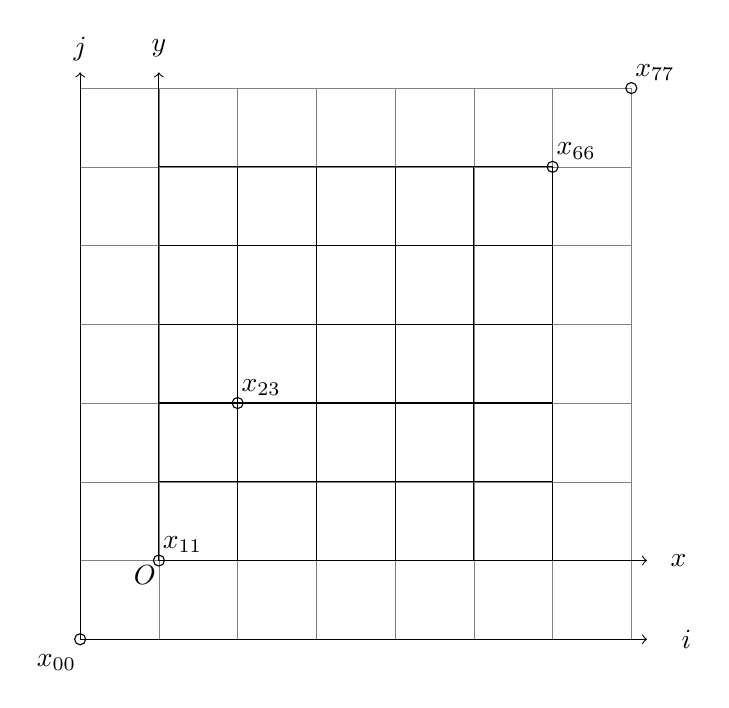
\begin{tikzpicture}
%grid
\draw[style=help lines] (-1,-1) grid +(7,7);
\draw (0,0) grid +(5,5);

%axes
\draw[->] (0,0) -- (xyz cs:x=0, y=6.2);
\draw (0,6.5) node {$y$};

\draw[->] (0,0) -- (xyz cs:x=6.2,y=0);
\draw (6.6,0) node {$x$};
\draw (-0.18,-0.18) node {$O$};

\draw[->] (-1,-1) -- (xyz cs:x=-1, y=6.2);
\draw (-1,6.5) node {$j$};

\draw[->] (-1,-1) -- (xyz cs:x=6.2, y=-1);
\draw (6.7,-1) node {$i$};

\draw (-1.3,-1.3) node {$x_{00}$};
\draw (-1,-1) circle (2pt);

\draw (0.3,0.2) node {$x_{11}$};
\draw (0,0) circle (2pt);

\draw (5.3,5.2) node {$x_{66}$};
\draw (5,5) circle (2pt);

\draw (6.3,6.2) node {$x_{77}$};
\draw (6,6) circle (2pt);

\draw (1.3,2.2) node {$x_{23}$};
\draw (1,2) circle (2pt);
\end{tikzpicture}
\caption{Mostra dos índices dos pontos do domínio e pontos imaginários\label{uma_malha}}
\end{figure}
\section{Conclusion}

O problema proposto inicialmente ainda não foi alcançado, que é trabalhar com a instabilidade de Saffman-Taylor com fluido magnético e, ou Anisotrópico. Antes de trabalhar com tal problema, teve-se uma etapa inicial que demandou um certo trabalho. Essa primeira etapa consistiu do estudo da resolução de equações diferenciais parciais, por meio de sua discretização e codificação em um programa de computador.

Foi bem sucedida a resolução das equações de Laplace e Poisson numa malha quadrada, pelos métodos direto e iterativo, com diferenças finitas. No caso da equação de Poisson, ainda teve-se a resolução bem sucedida com condições de fronteira de Neumann, que seria essencial para trabalhar com a pressão na equação de Navier Stokes.

O trabalho foi um aprendizado razoavelmente complexo, e que teve muitas consequências positivas. As habilidades de programação de programas numéricos pelo aluno aumentaram bastante, na realidade, de qualquer programa, pelo fato de se ter treinado bastante o uso do git e da ferramenta de compilação cmake. Apesar da programação ainda ser um problema, pela complexidade do programa, o código\footnote{Código está acessível online em https://github.com/ataias/ff} está muito mais organizado do que se esperava, e pra isso ele foi refeito algumas vezes.

O programa para resolver a equação de Navier Stokes na malha escalonada está sendo implementado e espera-se obter resultados nas etapas posteriores deste projeto.

\section*{Acknowledgments}

Primeiramente agradeço a Deus pela oportunidade de ter feito parte deste trabalho. Agradeço também ao professor Yuri Dumaresq pelas orientações e ânimo no ensino que eu vi nele e que também me animaram na resolução destes problemas numéricos. Agradeço também ao CNPq pela bolsa de incentivo à pesquisa.
%
%\begin{thebibliography}{4}
%\bibitem{magnetic_fluids} Rosensweig, R.E. 1987. Magnetic Fluids. Annu. Rev. Fluid Mech. 19:437-461.
%\bibitem{immersed_boundary_methods} Mittal R, Iaccarino G. 2005. Immersed Boundary Methods. Annu. Rev. Fluid Mech. 37:239-61.
%\bibitem{immersed_boundary_methods2} Perkin, C. S. 2002. The immersed boundary method. Act. Numerica p. 479:517
%\bibitem{notas_de_aula_john} Hinch, E.J. Lecture notes on Computational Fluid Dynamics: Part I - A first problem. 
%\bibitem{fingering} Babchin, A., Brailovsky, I. Gordon, P., Sivashinsky, G. Fingering instability in immiscible displacement. . Phys. Rev. E , 77, 026301, (2008).
%\bibitem{time_splitting} Chorin, A. J. A numerical method for solving incompressible viscous flow problems. J. Computational Physics, v. 2, 1967, p. 12
%\end{thebibliography}

\bibliographystyle{plain}
\bibliography{pibic}


\end{document}
